% Options for packages loaded elsewhere
\PassOptionsToPackage{unicode}{hyperref}
\PassOptionsToPackage{hyphens}{url}
\PassOptionsToPackage{dvipsnames,svgnames,x11names}{xcolor}
%
\documentclass[
]{book}
\usepackage{amsmath,amssymb}
\usepackage{lmodern}
\usepackage{iftex}
\ifPDFTeX
  \usepackage[T1]{fontenc}
  \usepackage[utf8]{inputenc}
  \usepackage{textcomp} % provide euro and other symbols
\else % if luatex or xetex
  \usepackage{unicode-math}
  \defaultfontfeatures{Scale=MatchLowercase}
  \defaultfontfeatures[\rmfamily]{Ligatures=TeX,Scale=1}
\fi
% Use upquote if available, for straight quotes in verbatim environments
\IfFileExists{upquote.sty}{\usepackage{upquote}}{}
\IfFileExists{microtype.sty}{% use microtype if available
  \usepackage[]{microtype}
  \UseMicrotypeSet[protrusion]{basicmath} % disable protrusion for tt fonts
}{}
\makeatletter
\@ifundefined{KOMAClassName}{% if non-KOMA class
  \IfFileExists{parskip.sty}{%
    \usepackage{parskip}
  }{% else
    \setlength{\parindent}{0pt}
    \setlength{\parskip}{6pt plus 2pt minus 1pt}}
}{% if KOMA class
  \KOMAoptions{parskip=half}}
\makeatother
\usepackage{xcolor}
\usepackage{longtable,booktabs,array}
\usepackage{calc} % for calculating minipage widths
% Correct order of tables after \paragraph or \subparagraph
\usepackage{etoolbox}
\makeatletter
\patchcmd\longtable{\par}{\if@noskipsec\mbox{}\fi\par}{}{}
\makeatother
% Allow footnotes in longtable head/foot
\IfFileExists{footnotehyper.sty}{\usepackage{footnotehyper}}{\usepackage{footnote}}
\makesavenoteenv{longtable}
\usepackage{graphicx}
\makeatletter
\def\maxwidth{\ifdim\Gin@nat@width>\linewidth\linewidth\else\Gin@nat@width\fi}
\def\maxheight{\ifdim\Gin@nat@height>\textheight\textheight\else\Gin@nat@height\fi}
\makeatother
% Scale images if necessary, so that they will not overflow the page
% margins by default, and it is still possible to overwrite the defaults
% using explicit options in \includegraphics[width, height, ...]{}
\setkeys{Gin}{width=\maxwidth,height=\maxheight,keepaspectratio}
% Set default figure placement to htbp
\makeatletter
\def\fps@figure{htbp}
\makeatother
\setlength{\emergencystretch}{3em} % prevent overfull lines
\providecommand{\tightlist}{%
  \setlength{\itemsep}{0pt}\setlength{\parskip}{0pt}}
\setcounter{secnumdepth}{5}
\usepackage{booktabs}
\ifLuaTeX
  \usepackage{selnolig}  % disable illegal ligatures
\fi
\usepackage[]{natbib}
\bibliographystyle{apalike}
\IfFileExists{bookmark.sty}{\usepackage{bookmark}}{\usepackage{hyperref}}
\IfFileExists{xurl.sty}{\usepackage{xurl}}{} % add URL line breaks if available
\urlstyle{same} % disable monospaced font for URLs
\hypersetup{
  pdftitle={Computational Thinking through Modular Sounds Synthesis},
  pdfauthor={Andrew M. Olney},
  colorlinks=true,
  linkcolor={Maroon},
  filecolor={Maroon},
  citecolor={Blue},
  urlcolor={blue},
  pdfcreator={LaTeX via pandoc}}

\title{Computational Thinking through Modular Sounds Synthesis}
\author{Andrew M. Olney}
\date{2022-08-29}

\begin{document}
\maketitle

{
\hypersetup{linkcolor=}
\setcounter{tocdepth}{1}
\tableofcontents
}
\hypertarget{welcome}{%
\chapter*{Welcome}\label{welcome}}
\addcontentsline{toc}{chapter}{Welcome}

This is the official website for ``Computational Thinking through Modular Sound Synthesis''. This book will teach you computational thinking through modular sound synthesis (hereafter \emph{modular}). You'll learn how to trigger sounds, create sounds, and modify sounds to solve specific sound design problems and create compositions. Along the way, you'll learn computational thinking practices that transcend modular and can be applied to a variety of problem-solving domains, but which are particularly relevant to information processing domains like computing.

If you're wondering whether this is a book about computational thinking, or a book about modular, the answer is both: on the surface, most content is about modular, but computational thinking is a style of thinking reflected in the presentation of the material and gives it additional coherence. As you work through the book, you'll become more proficient in computational thinking practices like decomposition, algorithmic design, evaluation of solutions, pattern recognition, and abstraction.

This book is \emph{interactive}, which is why it is an e-book rather than a paper book. Throughout you will encounter examples, simulations, and exercises that run in your browser to demonstrate and reinforce key concepts. Don't skip the interactive activities!


\includegraphics{images/by-nc-nd.png}

This website is free to use and is licensed under the \href{https://creativecommons.org/licenses/by-nc-nd/4.0/}{Creative Commons Attribution-NonCommercial-NoDerivs 4.0 License}.

\hypertarget{introduction}{%
\chapter{Introduction}\label{introduction}}

\hypertarget{why-this-book}{%
\section{Why this book?}\label{why-this-book}}

Let's start with why I'm writing it.
I got into electronic music in the 1990s when I lived in London but never transitioned from DJing to making music, though several of my friends did.
A few years ago, they started talking about modular, and in talking to them and trying to find out more about it, I realized a few things:

\begin{itemize}
\tightlist
\item
  The best books (to me) were from the 1970s and 1980s\footnote{Old books that I like are \citet{Crombie1982} and \citet{Strange1983}. Newer books of note are \citet{Bjoern2018}, which gives a great overview of module hardware and history, \citet{Eliraz2022}, which gives a broader overview of issues related to musical equipment and production, and \citet{Dusha2020}, which gives a modern but briefer introduction to modular than the older books. There are also some online courses (paid), but since I haven't taken them, I'm not listing them here.}
\item
  Modular synthesis is really well aligned with \emph{computational thinking}
\end{itemize}

If you've never heard of computational thinking and/or modular, that last point won't make a lot of sense, so let's break it down.

Modular sound synthesis (modular) creates sound by connecting modules that each perform some function on sound.
Different sounds are created by combining modules in different ways.

Computational thinking creates runnable models to solve a problem or answer a question.
Models can be scientific models (e.g.~meteorology), statistical models (e.g.~statistics/data science), computation models (computer science), and perhaps other kinds of models.

How are they connected?
Modular involves computational thinking when we:

\begin{itemize}
\tightlist
\item
  Simulate an instrument by reverse engineering its sound
\item
  Create new sounds based on models of signal processing
\end{itemize}

\textbf{Why should you read this book?}
This book is about modular, but it approaches modular in a way that highlights computational thinking.
I believe this deeper approach to modular will help you do more with modular, other synthesizers, and studio production tools.
Additionally, the computational thinking approach should help accelerate your learning of computational-thinking domains in the future.
Since computational thinking involves problem solving, this book is full of interactive activities that will let you hone your modular skills - something you won't find in most books!

The next sections give some background on computational thinking and modular to better explain where this book is coming from.

\hypertarget{computational-thinking}{%
\section{Computational thinking}\label{computational-thinking}}

\citet{Tedre2016} present a nice overview of the history of computational thinking.
Here's a brief summary.

When the field of computing was taking off in the 1950s, there was interest and discussion about how it was different from other fields (e.g.~math).
One argument was that computing involved \emph{algorithmic thinking}, which is designing algorithms to solve problems (cf.~programming), and this kind of thinking was unique to computing.
Some even thought that this kind of thinking could improve thinking generally.

\emph{Computational thinking} appears to have been coined in the 1980s by Seymour Papert and popularized in his book \emph{Mindstorms} \citep{Papert1980}.
Papert was a mathematician by training, and his approach was much broader than the algorithmic thinking approach that came before.
Papert's approach was empirical and embraced model building, which he implemented using simulated microworlds containing robots (LEGO Mindstorms takes its name from this work).
It was revolutionary in its time and received a lot of attention from educators and policy makers of widely different backgrounds.

Unfortunately, today it's very hard to get agreement on what computational thinking is, so definitions tend to be squishy.
This is likely due to the widespread use of computers and the tendency for everyone to frame computational thinking in terms of what \emph{they} do with computers.
Some want to reduce it to computer literacy, others to basic programming, and yet others to discovery learning with computers, etc.

I take a more unified view of computational thinking based on model building and problem solving.
I define computational thinking as building a \emph{runnable} model to solve a problem:

\begin{itemize}
\tightlist
\item
  For an algorithmic problem, this is a \href{https://en.wikipedia.org/wiki/Model_of_computation}{model of computation} (the original computer science view)
\item
  For data science/statistics, this is a \href{https://en.wikipedia.org/wiki/Statistical_model}{statistical model}
\item
  For general scientific fields, this is a \href{https://en.wikipedia.org/wiki/Scientific_modelling}{scientific model} of a phenomenon or process
\end{itemize}

The model doesn't need to run on a computer, but to be a runnable model, it needs to be mechanistic.
One of my favorite examples of a non-computer model is MENACE \citep{Michie1963}, which plays tic-tac-toe (AKA noughts and crosses).
MENACE plays tic-tac-toe using matchboxes full of colored beads as shown in Figure \ref{fig:menace}.
Each possible board position (starting with a blank board) is represented by a matchbox, and each move is represented by one of nine colored beads.
To make a move, a human assistant selects the correct box for the current board position and randomly samples a colored bead, which determines where MENACE makes its move.
If MENACE wins the game, the chosen bead from each box is replaced along with extra beads of the same color, and if MENACE loses, the chosen bead is removed.
Over time, these bead adjustments make winning moves more likely and losing moves less likely.



\begin{figure}
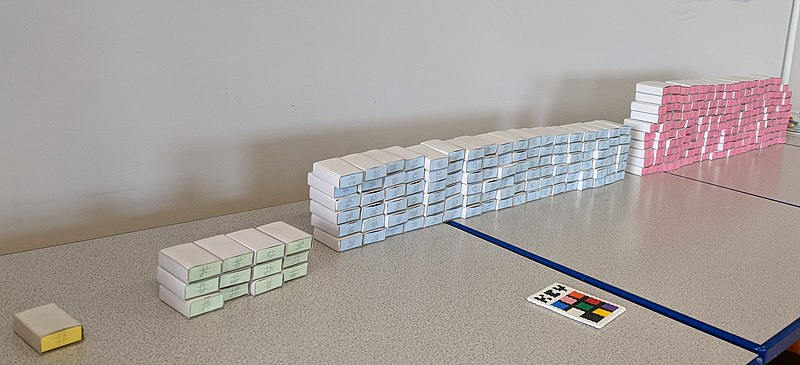
\includegraphics[width=1\linewidth]{images/800px-Mscroggs-MENACE-cropped} \caption{Machine Educable Noughts and Crosses Engine (MENACE). Each matchbox corresponds to a possible board position and is full of colored beads corresponding to moves. The color key in the foreground shows the board location indicated by each colored bead. Image \href{https://commons.wikimedia.org/wiki/File:Mscroggs-MENACE-cropped.jpg}{© Matthew Scroggs/CC-BY-SA-4.0}.}\label{fig:menace}
\end{figure}

MENACE is a nice example of computational thinking without computers because algorithmic game playing has a long history in computer science and AI.
However MENACE is not ``an exception to the rule'' - teaching computer science without computers has been part of the model curriculum for almost 20 years \citep{Tucker2003, Bell2021}.
We really don't need computers for computational thinking!

So how do we \emph{learn} to build runnable models to solve problems (i.e., how do we learn computational thinking)?
Well, models are made of interacting elements, so we need to learn those elements, and we need to learn how the elements interact.

Once we know those things, we can customize general problem solving, which has the same basic steps \citep{Polya2004}:

\begin{itemize}
\tightlist
\item
  Understand the problem
\item
  Make a plan
\item
  Implement the plan
\item
  Evaluate the solution
\end{itemize}

For any new domain, the big things to learn are the ``understand the problem'' and the ``make a plan'' steps of problem solving.
That's the approach of this book - for the domain of modular synthesis.

\hypertarget{modular-synthesis}{%
\section{Modular synthesis}\label{modular-synthesis}}

While we can pinpoint the invention of modular synthesis with some precision, it is useful to consider it in a broader context.
This section briefly overviews the history of synthesis and how modular fits into it.

Humans have long been interested in musical instruments that incorporate automation or in reproducing sounds by mechanical means.
Wind chimes, which play a series of notes when disturbed by wind, appeared in the historical record thousands of years ago.
Even before the complete electrification of instruments (synthesizers are electric by definition), there were numerous attempts to partially automate or model sounds, such as barrel organs, player pianos, or speech synthesis using bellows \citep{Dudley1950} as shown in Figure \ref{fig:kemplen-machine}.



\begin{figure}
\centering
\includegraphics{downloadFigs4latex/kemplen-machine.jpg}
\caption{\label{fig:kemplen-machine}\href{https://youtu.be/k_YUB_S6Gpo?start=21}{YouTube video} of Wolfgang von Kempelen's speaking machine circa 1780. Image \href{https://www.youtube.com/user/Quintatoen}{© Fabian Brackhane}.}
\end{figure}

Consider the difference between wind chimes or a player piano and this speaking machine.
Neither of the former is a model of the sound but rather uses mechanical means to trigger the sound (later we will refer to this as sequencing).
In contrast, the speaking machine is a well-considered model of the human speech mechanism.

Synthesizers using electricity appeared in the late 19th century.\footnote{There is some difference of opinion on what qualifies as usage of electricity in this context. For a fuller history of synthesizers, see \url{https://120years.net/wordpress/}}
Patents were awarded just a few years apart to Elisha Gray, whose synthesizer comprised simple single note oscillators and transmitted over the telegraph, and Thaddeus Cahill, whose larger Telharmonium could sound like an organ or various wood instruments but weighed 210 tons!

The modular synthesizer was developed by Harald Bode from 1959-1960 \citep{Bode1984}, and this innovation quickly spread to other electronic music pioneers like Moog and Buchla.
The key idea of modular is flexibility.
This is achieved by refactoring aspects of synthesis (i.e.~functions on sound) into a collection of modules.
These modules may then be combined to create a certain sound by patching them together and adjusting module parameters (e.g.~by turning knobs or adjusting sliders).
An example modular synthesizer is shown in Figure \ref{fig:serge-modular}.



\begin{figure}
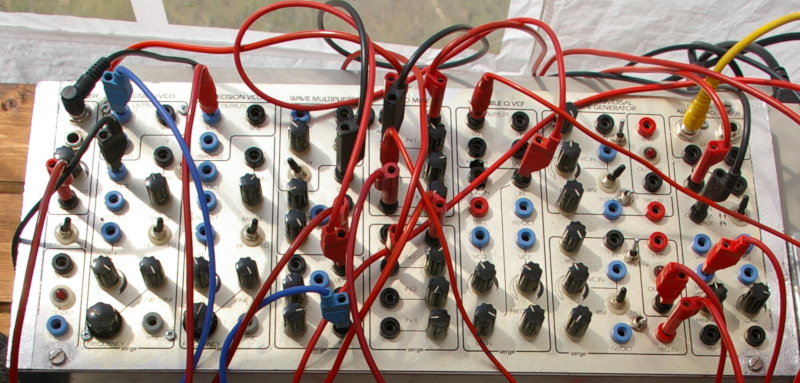
\includegraphics[width=1\linewidth]{images/Serge_Modular,_Norbergfestival_2007_cropped} \caption{A Serge modular system based on a 1970s design. Each module is labeled at the top edge, e.g.~``Wave Multiplier,'' and extends down to the bottom edge in a column. Note that although the modules have the same height, they have different widths. Image \href{https://commons.wikimedia.org/wiki/File:Serge_Modular,_Norbergfestival_2007.jpg}{© mikael altemark/CC-BY-2.0}.}\label{fig:serge-modular}
\end{figure}

In the 1970s, \emph{semi-modular} synthesizers were developed that did not require patching to make a sound.
Instead, semi-modulars were pre-set with an invisible default patch, meaning that the default patch wiring was internal and not visible to the user.
Users could then override this default patch by plugging in patch cables.
Most semi-modulars from this period also included an integrated keyboard.
Arguably, theses changes made semi-modulars more approachable to typical musicians.
An example semi-modular synthesizer is shown in Figure \ref{fig:semi-modular}.



\begin{figure}
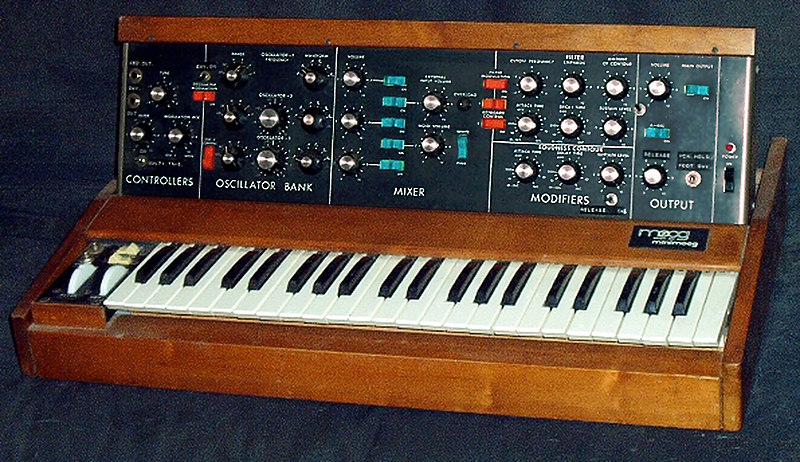
\includegraphics[width=1\linewidth]{images/800px-Minimoog} \caption{A Minimoog semi-modular system from the 1970s. Patch points are primarily on the top edge and hidden from view. Image \href{https://commons.wikimedia.org/wiki/File:Minimoog.JPG}{public domain}.}\label{fig:semi-modular}
\end{figure}

Digital technology began replacing the analog technology of synthesizers in the 1980s.
As a result, synthesizers got smaller and cheaper.
Digital synthesizers made increasing use of preset sounds so that most users never needed to create custom sounds.
In comparison to digital synthesizers, modular synthesizers were more expensive and harder to use.
An example digital synthesizer is shown in Figure \ref{fig:dx7}.



\begin{figure}
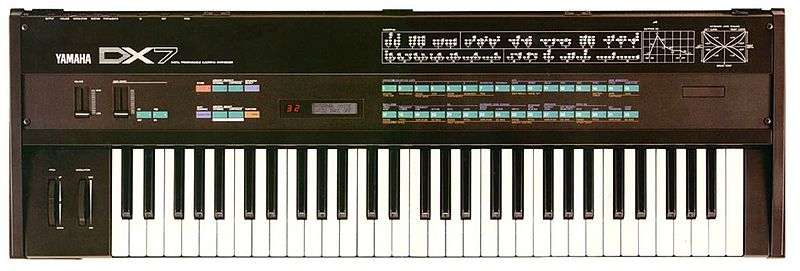
\includegraphics[width=1\linewidth]{images/YAMAHA_DX7} \caption{A Yamaha DX7 from the 1980s. Note the menu-based interface and relative lack of controls compared to modular and semi-modular synthesizers. Image \href{https://commons.wikimedia.org/wiki/File:YAMAHA_DX7.jpg}{public domain}.}\label{fig:dx7}
\end{figure}

By the 1990s the digital transformation was complete, such that computers could be used to create and produce music in software.
Although computers were still relatively expensive at this time, they provided an all-in-one solution that included editing, mixing, and other production aspects.
Over the next few decades as personal computers and portable computing devices became common household items, the costs associated with computer-based music making became dominated by the cost of software and associated audio and \href{https://en.wikipedia.org/wiki/MIDI}{MIDI} interfaces.
Figure \ref{fig:logic} shows digital audio workstation (DAW) software commonly used in music production.



\begin{figure}
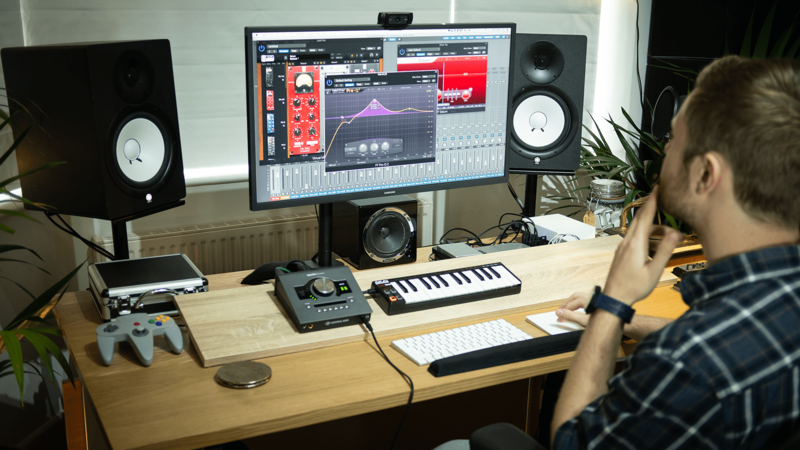
\includegraphics[width=1\linewidth]{images/800px-Logic_PRO_X_Tutorial} \caption{Logic Pro digital audio workstation software. Additional functionality is provided by 3rd-party plugins showing as additional windows on the screen. In the foreground are an audio interface and a MIDI keyboard used for recording/playing audio and entering note information respectively. Image \href{https://commons.wikimedia.org/wiki/File:Logic_PRO_X_Tutorial.png}{© Musicianonamission/CC-BY-SA-4.0}.}\label{fig:logic}
\end{figure}

The computer-centric approach dominated synthesis for a decade or more, but by the 2010s, improved electronics manufacturing, smartphone technology, and the open-source movement led to lower cost modular synthesizers.
Additionally, the Eurorack standard \citep{DoepferMusikelektronik2022, DoepferMusikelektronik2022a} was widely adopted, leading to +10,000 interoperable modules.\footnote{\url{https://www.modulargrid.net/}}
As a result, modular synthesis saw a resurgence in popularity.
Figure \ref{fig:eurorack} shows a Eurorack modular synthesizer.



\begin{figure}
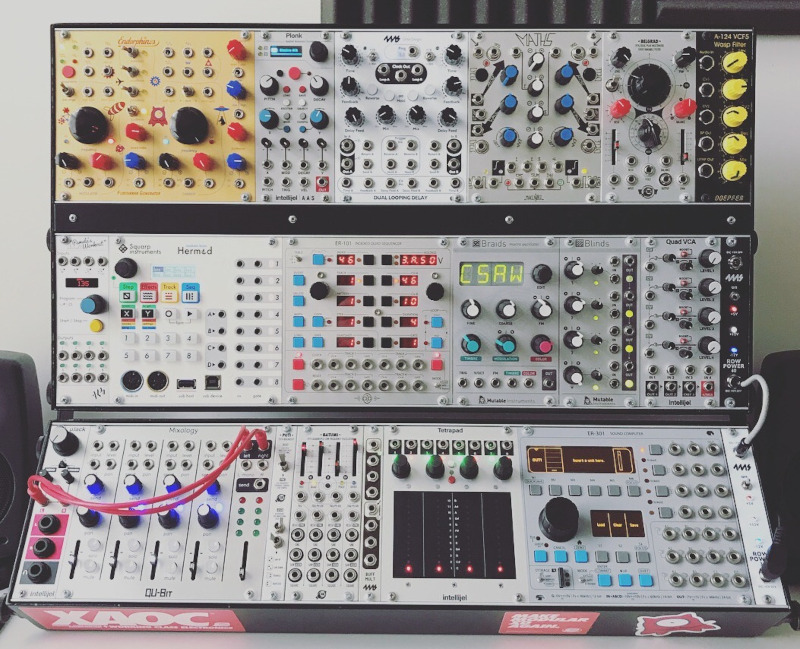
\includegraphics[width=1\linewidth]{images/Eurorack_Modular_Synthesizer-cropped} \caption{A Eurorack modular synthesizer. The different modules designs and logos reflect the adoption of the Eurorack standard which makes modules from different manufacturers interoperable. Image \href{https://commons.wikimedia.org/wiki/File:Eurorack_Modular_Synthesizer.jpg}{© Paul Anthony/CC-BY-SA-4.0}.}\label{fig:eurorack}
\end{figure}

It is perhaps surprising that some 60 years after its creation, modular synthesis is more popular than ever.
One possible reason is the reduction in price over time, shown in Table \ref{tab:price}.
However, other trends seem to be at work.
While the modular synthesizer was simplified for wider adoption early in its history, first with semi-modular and later with digital synthesizers, the culmination of this trend led to large preset and sample banks that transformed the task of creating a specific sound to searching for a pre-made sound.
It's plausible that as the search for sounds became more intensive, the time savings of presets diminished, making the modular approach more attractive.
An intersecting trend is a commonly-expressed dissatisfaction with using computers for every aspect of music making and a corresponding return to hardware instruments, including modular.

\begin{longtable}[]{@{}lll@{}}
\caption{\label{tab:price} The cost of modular, semi-modular, and computer synthesizers over time. Prices are in 2022 dollars.}\tabularnewline
\toprule()
Decade & Synthesizer & Cost \\
\midrule()
\endfirsthead
\toprule()
Decade & Synthesizer & Cost \\
\midrule()
\endhead
1960s & Moog modular synthesiser & \$96,000 \\
1970s & Minimoog semi-modular & \$10,000 \\
1980s & Yamaha DX7 & \$6,000 \\
1990s & Gateway computer with Cubase & \$8,000 \\
2010s & ALM System Coupe modular & \$2,400 \\
\ldots{} & VCVRack virtual modular & Free \\
\bottomrule()
\end{longtable}

Earlier in this chapter, I argued that a computational thinking approach to modular could help with other synthesizers and studio production tools.
Hopefully this brief history helps explain why: modular represents the building blocks of synthesis that later approaches have appropriated and presented in their own way.
A square wave oscillator in modular is fundamentally the same as that in another hardware synth or DAW software.
If you understand these building blocks in modular, you should understand them everywhere.

\hypertarget{moving-forward}{%
\section{Moving forward}\label{moving-forward}}

Our next stop is \emph{Sound} where the focus is to ``understand the problem''.
Chapter \ref{physics-and-perception} addresses both the physics of sound and our perception of it, which perhaps surprisingly, are not the same.
From there we move into sounds commonly found in music and their properties, ranging from harmonic sounds in Chapter \ref{harmonic-sounds} to inharmonic sounds like percussion in Chapter \ref{inharmonic-sounds}.

The remainder of the book alternates between learning model elements (modules), how they interact (patches), problem solving (sound design).
The progressive \emph{Modules} and \emph{Sound Design} sections build up from basic approaches to the more complex.
By the time we're done, you should have a good foundation to create patches to solve new sound design problems.

\hypertarget{part-sound}{%
\part{Sound}\label{part-sound}}

\hypertarget{physics-and-perception}{%
\chapter{Physics and Perception}\label{physics-and-perception}}

From the outset, it's important to understand that the physics of sound and how we perceive it are not the same.
This is a simple fact of biology.
Birds can see ultraviolet, and bats can hear ultrasound; humans can't do either.
Dogs have up to 40 times more olfactory receptors than humans and correspondingly have a much keener sense of smell.
We can only perceive what our bodies are equipped to perceive.

In addition to the limits of our perception, our bodies also \emph{structure} sensations in ways that don't always align with physics.
A good example of this is \href{https://en.wikipedia.org/wiki/Equal-loudness_contour}{equal loudness contours}.
As shown in Figure \ref{fig:elc}, sounds can appear equally loud to humans across frequencies even though the actual sound pressure level (a measure of sound energy) is not constant.
In other words, our hearing becomes more sensitive depending on the frequency of the sound.



\begin{figure}
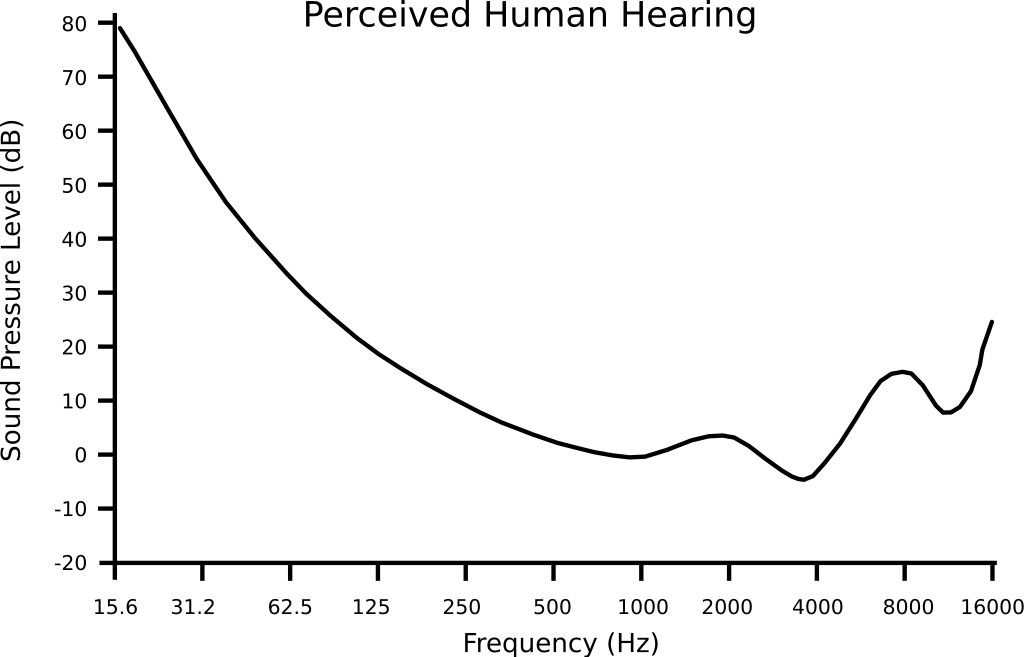
\includegraphics[width=1\linewidth]{images/Perceived_Human_Hearing.svg} \caption{An equal loudness contour showing improved sensitivity to frequencies between 500Hz and 4KHz, which approximately matches the range of human speech frequencies. Image \href{https://en.wikipedia.org/wiki/Psychoacoustics\#/media/File:Perceived_Human_Hearing.svg}{public domain}.}\label{fig:elc}
\end{figure}

Why do we need to understand the physics of sound \emph{and} perception of sound?
Although ultimately we hear the sounds we're going to make, the process of making the sounds is based in physics.
So we need to know how both the physics and perception of sound work, at least a bit.

\hypertarget{waves}{%
\section{Waves}\label{waves}}

Have you ever noticed a dust particle floating in the air, just randomly wandering around?
That random movement is known as Brownian motion, and it was shown by Einstein to be evidence for the existence of atoms - that you can see with your own eyes!
The movement is caused by air molecules\footnote{In what follows, we will ignore that air is a mixture of gases because it is irrelevant to the present discussion.} bombarding the dust particle from random directions, as shown in Figure \ref{fig:sim-brownian}.



\begin{figure}
\href{https://physics.bu.edu/~duffy/HTML5/brownian_motion.html}{\includegraphics[width=1\linewidth]{02-physics-perception_files/figure-latex/sim-brownian-1} }\caption{\href{https://physics.bu.edu/~duffy/HTML5/brownian_motion.html}{Simulation} of Brownian motion. Press \texttt{Pause} to stop the simulation. © Andrew Duffy/\href{https://creativecommons.org/licenses/by-nc-sa/4.0/}{CC-BY-NC-SA-4.0}.}\label{fig:sim-brownian}
\end{figure}

Air molecules are always whizzing around like this.
However, in much of the discussion below, we'll largely ignore this fact and focus instead on the properties of waves passing through air.

Amazingly, it is also possible to see sound waves moving through the air, using a technique called \href{https://en.wikipedia.org/wiki/Schlieren_photography}{Schlieren photography}.
Schlieren photography captures differences in air pressure, and sound is just a difference in air pressure that travels as a wave.



\begin{figure}
\includegraphics[width=1\linewidth]{downloadFigs4latex/firecracker-wave} \caption{\href{http://media.npr.org/assets/img/2014/01/21/cracker.gif}{Animation} of a firecracker exploding in slow motion, captured by Schlieren photography. Note the dark pressure wave that radiates outward. Image © Mike Hargather. Linked with \href{https://www.npr.org/about-npr/179876898/terms-of-use\#LinksNPRServices}{permission from NPR}.}\label{fig:firecracker-wave}
\end{figure}

The animation in Figure \ref{fig:firecracker-wave} shows a primary wave of sound corresponding to the explosion of the firecracker in slow motion, and we can see that wave radiate outwards from the explosion.



\begin{figure}
\centering
\includegraphics{downloadFigs4latex/slow-drum.jpg}
\caption{\label{fig:slow-drum}\href{https://www.youtube.com/watch?v=tM8WyhB6zYo}{Youtube video} of a slow motion drum hit. Watch how the drum head continues to move inward and outward after the hit. Image \href{https://www.youtube.com/channel/UCRZIyRiTD427A9dw3CBM4Fg}{© Boulder Drum Studio}.}
\end{figure}

Consider the slow motion drum hit in Figure \ref{fig:slow-drum}.
After the stick hits the drum head, the head first moves inward and then outward, before repeating the inward/outward cycle.
When the drum head moves inward, it creates more room for the surrounding air molecules, so the density of the air next to the drum head decreases (i.e.~it becomes less dense, because there is more space for the same amount of air molecules).
The decrease in density is called rarefaction.
When the drum head moves outward, it creates less room for the surrounding air molecules, so the density of the air next to the drum head increases (i.e.~it becomes more dense, because there is less space for the same amount of air molecules).
The increase in density is called compression.

You can see an analogous simulation of to the drum hit in Figure \ref{fig:sim-gas}.
If you add say 50 particles, grab the handle on the left, and move it to the right, the volume of the chamber decreases, and the pressure in the chamber goes up (compression).
Likewise, if you move the handle to the left, the volume of the chamber increases, and the pressure goes down (rarefaction).
In the drum example, when the stick hits the head and causes it to move inward, the volume of air above the head will rush in to fill that space (rarefaction), and when the head moves outward, the volume of air above the head will shrink (compression).



\begin{figure}
\href{https://phet.colorado.edu/sims/html/gas-properties/latest/gas-properties_en.html?screens=2}{\includegraphics[width=1\linewidth]{02-physics-perception_files/figure-latex/sim-gas-1} }\caption{\href{https://phet.colorado.edu/sims/html/gas-properties/latest/gas-properties_en.html?screens=2}{Simulation} of gas in a chamber. Simulation by \href{https://phet.colorado.edu/}{PhET Interactive Simulations}, University of Colorado Boulder, licensed under \href{https://creativecommons.org/licenses/by/4.0/}{CC-BY-4.0}.}\label{fig:sim-gas}
\end{figure}

Sound is a difference in air pressure that travels as a wave through compression and rarefaction.
We could see this with the firecracker example because the explosion rapidly heated and expanded the air, creating a pressure wave on the boundary between the surrounding air and the hot air.
However, as we've seen with the drum and will discuss in more detail later in this chapter, musical instruments are designed to create more than a single wave.
The Schlieren photography animation in Figure \ref{fig:schlieren-wave} is more typical of a musical instrument.



\begin{figure}
\includegraphics[width=1\linewidth]{downloadFigs4latex/schlieren-wave} \caption{\href{http://media.npr.org/assets/img/2014/01/21/speaker1.gif}{Animation} of a continuous tone from a speaker in slow motion, captured by Schlieren photography. Note the dark pressure wave that radiates outward. Image © Mike Hargather. Linked with \href{https://www.npr.org/about-npr/179876898/terms-of-use\#LinksNPRServices}{permission from NPR}.}\label{fig:schlieren-wave}
\end{figure}

The rings in Figure \ref{fig:schlieren-wave} represent compression (dark) and rarefaction (light) stages of the wave.
It is important to understand that air molecules aren't moving from the speaker to the left side of the image.
Instead, the wave is moving the entire distance, and the air molecules are only moving a little bit as a result of the wave.\footnote{The air molecules are moving randomly in general, so the simulation shows only the movement attributable to the effect of the wave.}

To see how this works, take a look at the simulation in Figure \ref{fig:sim-wave}.
Hit the green button to start the sound waves and then select the \texttt{Particles} radio button.
The red dots are markers to help you see how much the air is moving as a result of the wave.
As you can see, every red dot is staying in their neighborhood and only moving as a result of compression and rarefaction cycles.
If you select the \texttt{Both} radio button, you can see the outlines of waves on top of the air molecules.
Note how each red dot is moving back and forth between a white band and a dark band.
If you further select the \texttt{Graph} checkbox, you will see that the white bands in this simulation correpond to increases in pressure and the black bands correspond to decreases in pressure.
This type of graph is commonly used to describe waves, so make sure you feel comfortable with it before moving on.



\begin{figure}
\href{https://phet.colorado.edu/sims/html/waves-intro/latest/waves-intro_en.html?screens=2}{\includegraphics[width=1\linewidth]{02-physics-perception_files/figure-latex/sim-wave-1} }\caption{\href{https://phet.colorado.edu/sims/html/waves-intro/latest/waves-intro_en.html?screens=2}{Simulation} of sound waves. Simulation by \href{https://phet.colorado.edu/}{PhET Interactive Simulations}, University of Colorado Boulder, licensed under \href{https://creativecommons.org/licenses/by/4.0/}{CC-BY-4.0}.}\label{fig:sim-wave}
\end{figure}

\hypertarget{frequency-and-pitch}{%
\section{Frequency and pitch}\label{frequency-and-pitch}}

hz

\hypertarget{amplitude-and-loudness}{%
\section{Amplitude and loudness}\label{amplitude-and-loudness}}

db

\hypertarget{waveshape-and-timbre}{%
\section{Waveshape and timbre}\label{waveshape-and-timbre}}

\hypertarget{phase-and-phase}{%
\section{Phase and \ldots{} phase?}\label{phase-and-phase}}

You might think that we only need to understand how humans perceive sound and not the physics of it\ldots{}

\hypertarget{harmonic-sounds}{%
\chapter{Harmonic Sounds}\label{harmonic-sounds}}

\hypertarget{inharmonic-sounds}{%
\chapter{Inharmonic Sounds}\label{inharmonic-sounds}}

\hypertarget{part-fundamental-modules}{%
\part{Fundamental Modules}\label{part-fundamental-modules}}

\hypertarget{basic-concepts}{%
\chapter{Basic Concepts}\label{basic-concepts}}

\hypertarget{trigger}{%
\chapter{Trigger}\label{trigger}}

\hypertarget{create}{%
\chapter{Create}\label{create}}

\hypertarget{modify}{%
\chapter{Modify}\label{modify}}

\hypertarget{part-sound-design-1}{%
\part{Sound Design 1}\label{part-sound-design-1}}

\hypertarget{kick-cymbal}{%
\chapter{Kick \& Cymbal}\label{kick-cymbal}}

\hypertarget{lead-bass}{%
\chapter{Lead \& Bass}\label{lead-bass}}

\hypertarget{part-complex-modules}{%
\part{Complex Modules}\label{part-complex-modules}}

\hypertarget{trigger-1}{%
\chapter{Trigger}\label{trigger-1}}

\hypertarget{create-1}{%
\chapter{Create}\label{create-1}}

\hypertarget{modify-1}{%
\chapter{Modify}\label{modify-1}}

\hypertarget{part-sound-design-2}{%
\part{Sound Design 2}\label{part-sound-design-2}}

\hypertarget{minimoog-303}{%
\chapter{Minimoog \& 303}\label{minimoog-303}}

  \bibliography{book.bib,packages.bib}

\end{document}
